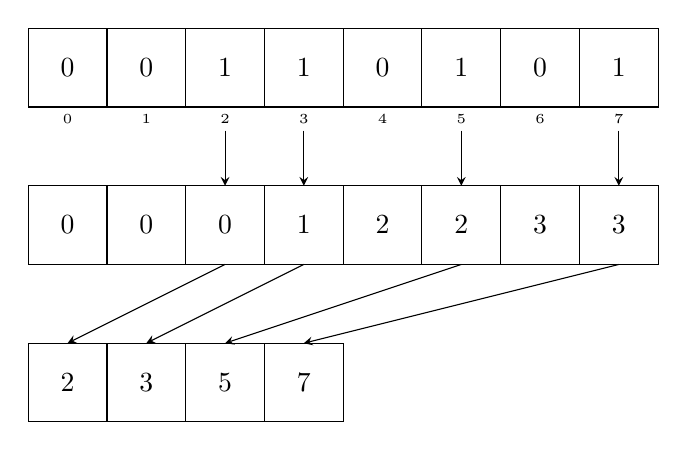
\begin{tikzpicture}[>=stealth]

\foreach \x/\val in {0/0,1/0,2/1,3/1,4/0,5/1,6/0,7/1}
{
  \draw (\x,0) rectangle ++(1,1);
  \draw node at (\x+0.5,0.5) {\val};
  \draw[font=\tiny] node at (\x+0.5,-0.15) {\x};
}

\foreach \x in {2,3,5,7}
{
  \draw[->] (\x+0.5,-0.3) -- ++(0,-0.7);
}

\foreach \x/\val in {0/0,1/0,2/0,3/1,4/2,5/2,6/3,7/3}
{
  \draw (\x,-2) rectangle ++(1,1);
  \draw node at (\x+0.5,-1.5) {\val};
}

\foreach \x/\val in {0/2,1/3,2/5,3/7}
{
  \draw (\x,-4) rectangle ++(1,1);
  \draw node at (\x+0.5,-3.5) {\val};
}

\foreach \x/\y in {0/2,1/3,2/5,3/7}
{
  \draw[->] (\y+0.5,-2) -- (\x+0.5, -3);
}
\end{tikzpicture}
